\documentclass[11pt,compress]{beamer}
% deactivate beamer navigation
%\setbeamertemplate{navigation symbols}{}
%\usepackage{geometry}
%\geometry{papersize={180mm, 135mm}, top=-1.5mm} % 210mm, 297mm
\usepackage{../style/lmu-lecture}
\setbeamertemplate{frametitle}{\expandafter\uppercase\expandafter\insertframetitle}

\usepackage{tikz}

\usepackage{setspace}



\AtBeginSection[]
{
  \begin{frame}<beamer>
    \frametitle{Introduction to Machine Learning}
  \begin{minipage}{\textwidth}
  %decrease linespacing to display all points
  \linespread{0.01}\selectfont
  \begin{spacing}{0.001}
  \begin{small}
  \tableofcontents[currentsection, subsectionstyle=hide]
  \end{small}
  \end{spacing}
  \end{minipage}
  \end{frame}
}
% includepdf slides, pagecommad will set counter for framenumber
\usepackage{pdfpages}
\includepdfset{trim=0mm 0mm 0mm 0mm, pagecommand={\global\setcounter{framenumber}{\value{page}}}}
% trim=0mm 6mm 0mm 0mm, offset=0 15,
% add footer:
  \usepackage{framed, color}
\usepackage{xcolor}
%\iffalse
\setbeamertemplate{footline}[text line]{%
  \noindent\hspace*{\dimexpr-\oddsidemargin-1in\relax}%
  \colorbox{white}{
    \makebox[\dimexpr\paperwidth-2\fboxsep\relax]{
      \color{black}
      \begin{minipage}[c][4.5ex][c]{0.5\linewidth}
      \secname
      \end{minipage}
      \hfill\begin{minipage}[c][4.5ex][c]{0.5\linewidth}
      \flushright
      \insertframenumber{}~/~\inserttotalframenumber~~
        \end{minipage}
    }}%
  \hspace*{-\paperwidth}
}
%\fi


\title{
  \hspace{-0.5cm}\centerline{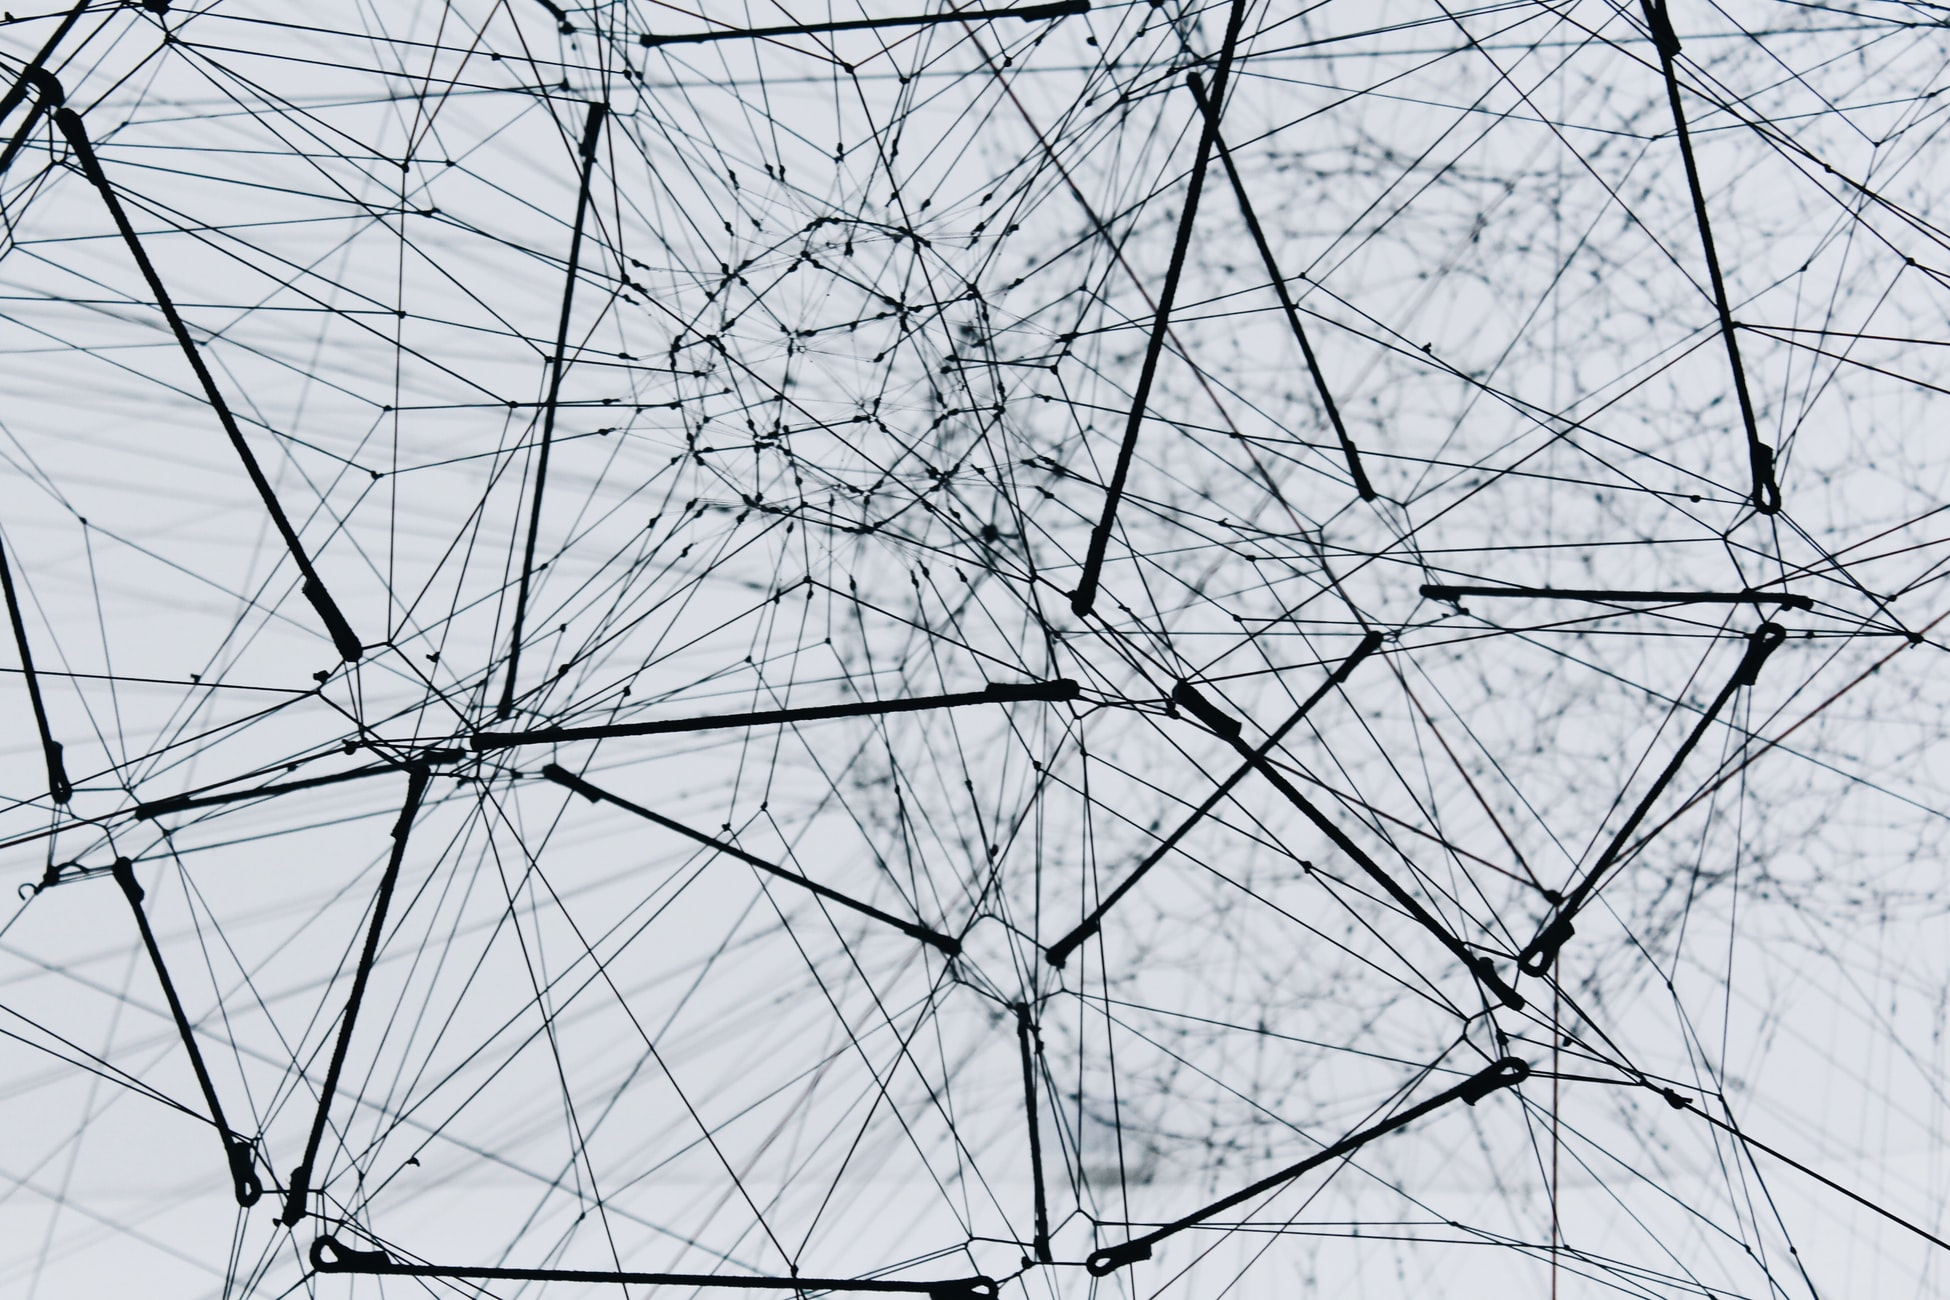
\includegraphics[width=1.05\paperwidth,keepaspectratio, trim={0 15cm 0 5cm}, clip]{titlepage.jpg}}
  \medskip
  Supervised Learning \\
  \medskip
  \small All slides
  \vspace{-1.5cm}
}



\begin{document}
\setbeamercolor{background canvas}{bg=}

\begin{frame}[noframenumbering,plain]
\maketitle
\end{frame}


% General remark: hyperlinks in included pdfs are not clickable anymore in the combined pdf

% Include tuning lecture slides
\section{Advanced Risk Minimization}
%% needs to be filled!!
% slides-advriskmin-risk-minimizer
% slides-advriskmin-pseudo-residuals
% slides-advriskmin-regression-l2
% slides-advriskmin-regression-l1
% slides-advriskmin-regression-further-losses
% slides-advriskmin-cassification-01
% slides-advriskmin-cassification-bernoulli
% slides-advriskmin-cassification-brier
% slides-advriskmin-cassification-furtherlosses
% slides-advriskmin-max-likelihood-l2
% slides-advriskmin-max-likelihood-other
% slides-advriskmin-losses-properties

%- slides-evaluation-intro

\subsection{Risk Minimizers}
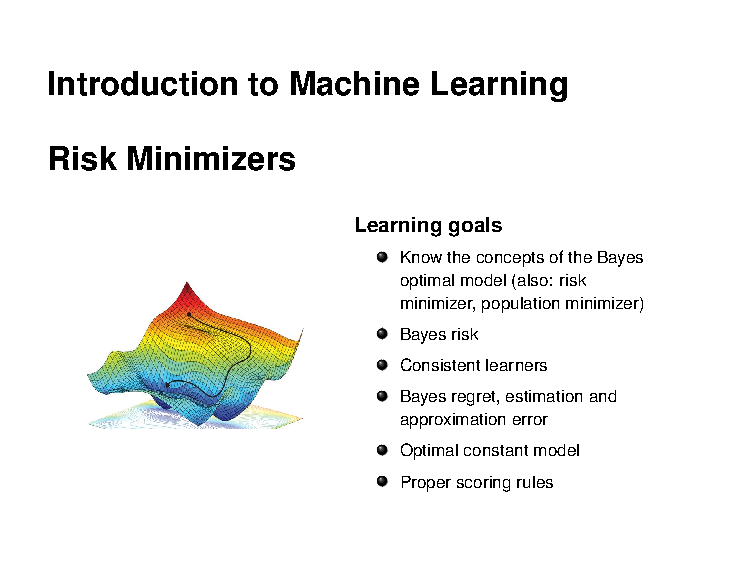
\includepdf[pages=-]{../slides-pdf/slides-advriskmin-risk-minimizer.pdf}

\subsection{Pseudo-Residuals}
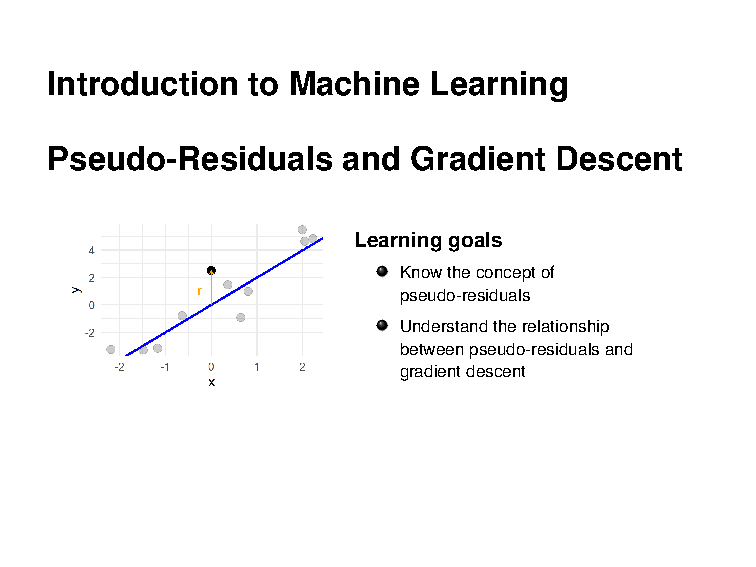
\includepdf[pages=-]{../slides-pdf/slides-advriskmin-pseudo-residuals.pdf}

\subsection{L2-loss}
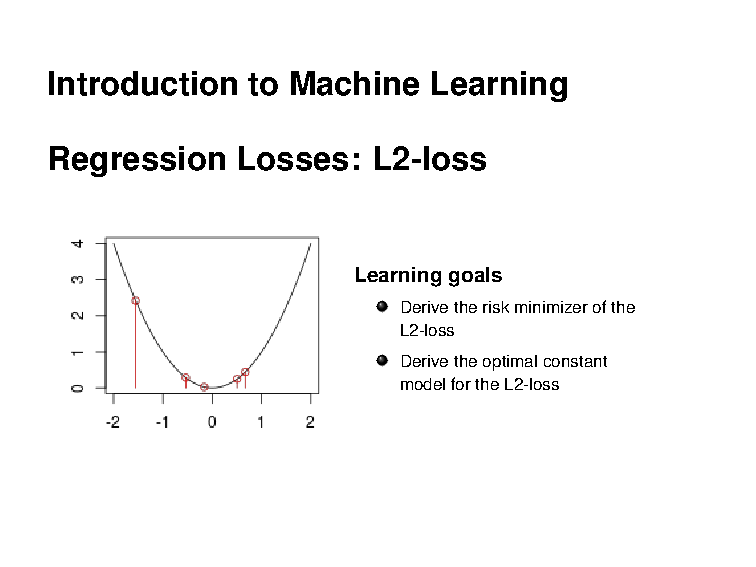
\includepdf[pages=-]{../slides-pdf/slides-advriskmin-regression-l2.pdf}

\subsection{L1-loss}
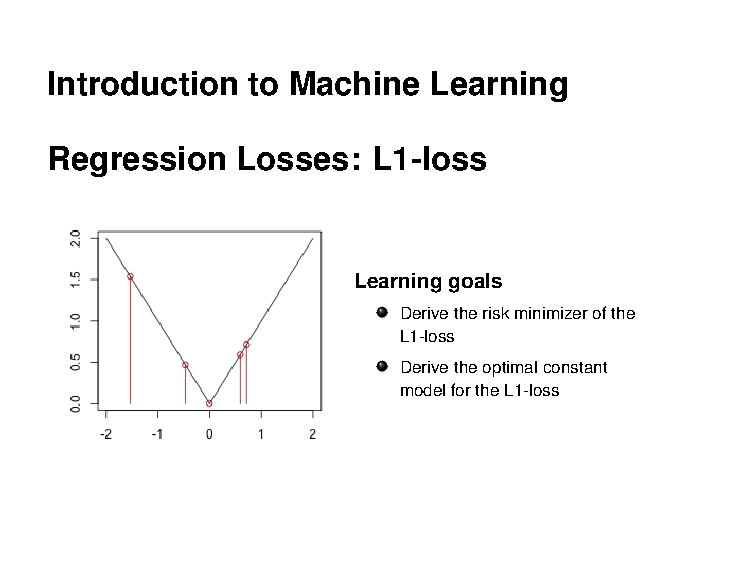
\includepdf[pages=-]{../slides-pdf/slides-advriskmin-regression-l1.pdf}

\subsection{Advanced Regression Losses}
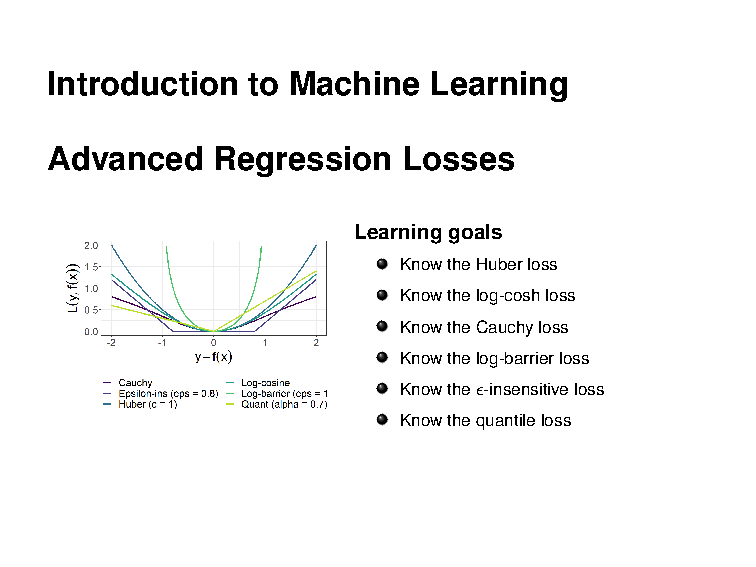
\includepdf[pages=-]{../slides-pdf/slides-advriskmin-regression-further-losses.pdf}

\subsection{0-1-loss}
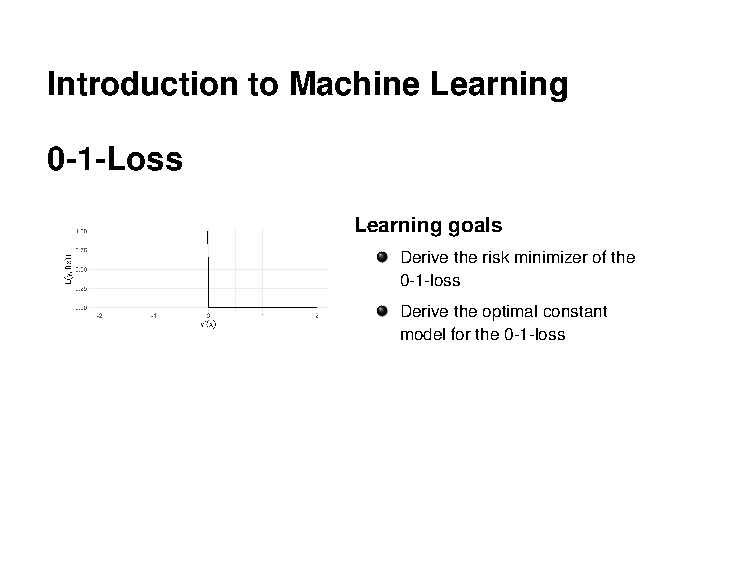
\includepdf[pages=-]{../slides-pdf/slides-advriskmin-classification-01.pdf}

\subsection{Bernoulli Loss}
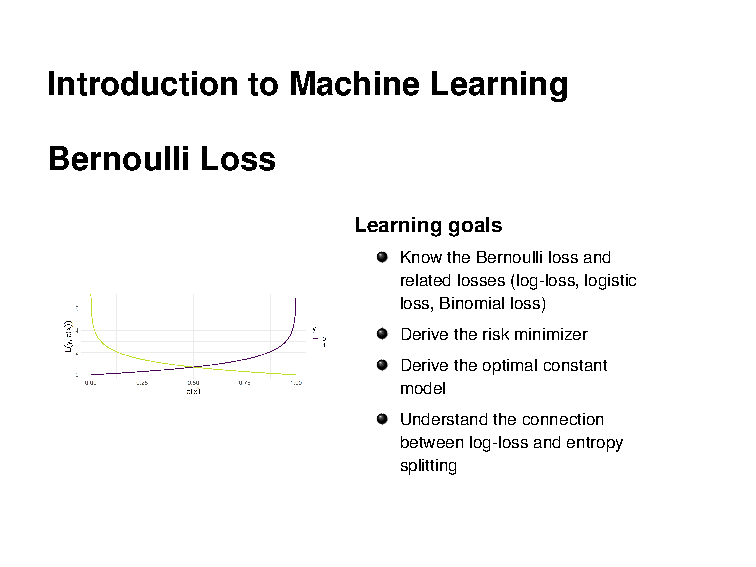
\includepdf[pages=-]{../slides-pdf/slides-advriskmin-classification-bernoulli.pdf}

\subsection{Brier Score}
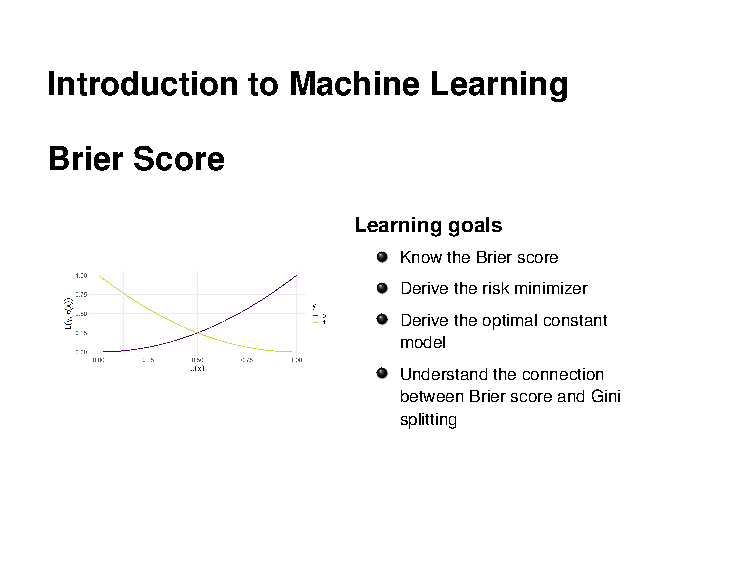
\includepdf[pages=-]{../slides-pdf/slides-advriskmin-classification-brier.pdf}

\subsection{Advanced Classification Losses}
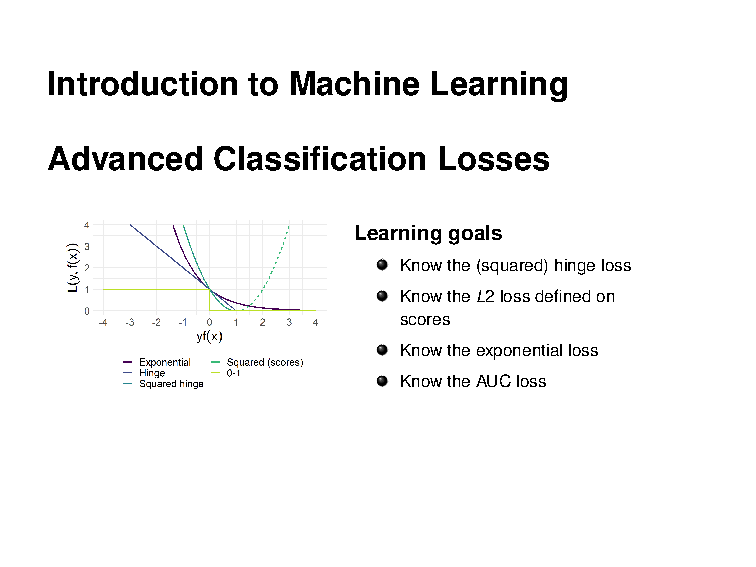
\includepdf[pages=-]{../slides-pdf/slides-advriskmin-classification-furtherlosses.pdf}

\subsection{Maximum Likelihood Estimization vs. Empirical Risk Minimization I}
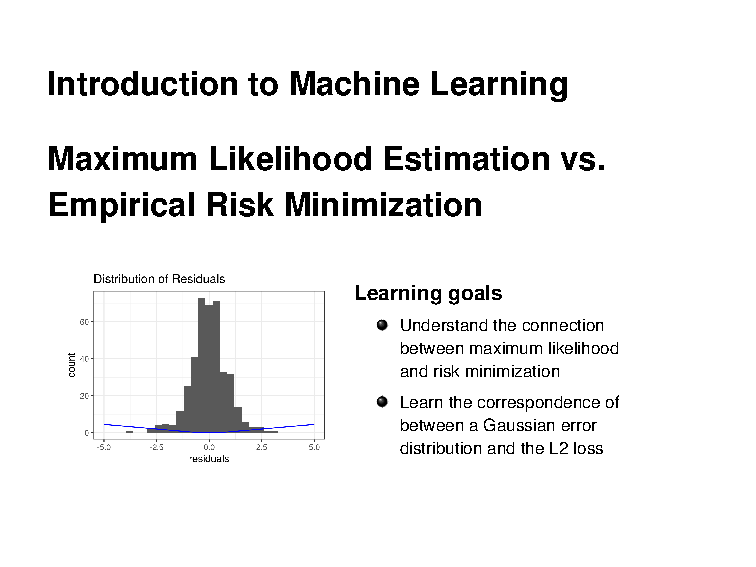
\includepdf[pages=-]{../slides-pdf/slides-advriskmin-max-likelihood-l2.pdf}

\subsection{Maximum Likelihood Estimization vs. Empirical Risk Minimization II}
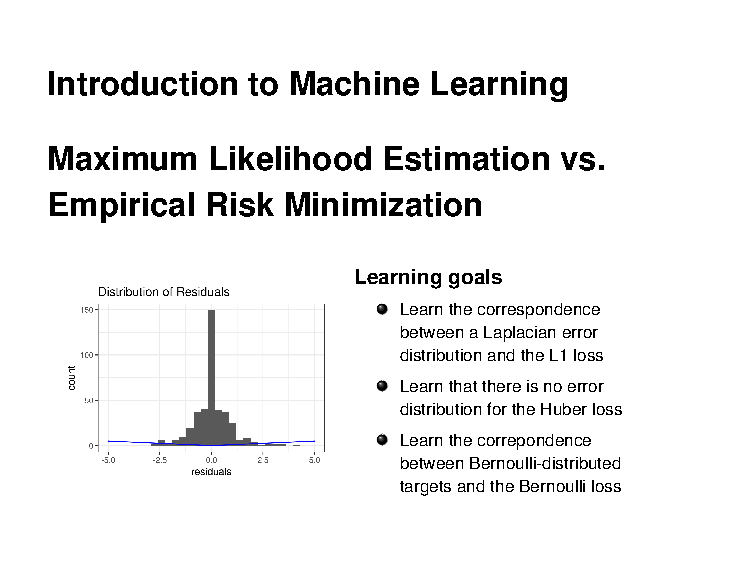
\includepdf[pages=-]{../slides-pdf/slides-advriskmin-max-likelihood-other.pdf}

\subsection{Loss Properties}
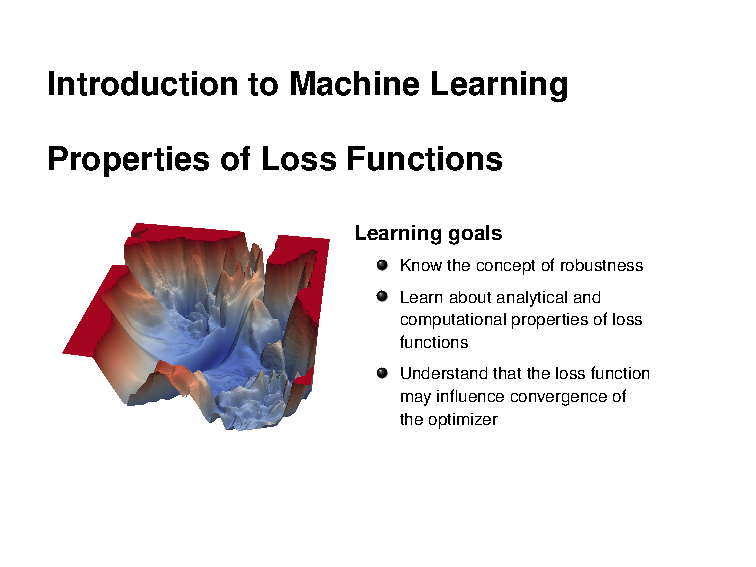
\includepdf[pages=-]{../slides-pdf/slides-advriskmin-losses-properties.pdf}



\section{Multiclass Classification}
%Suggested order of slides
% slides-mc-losses
% slides-mc-softmax-regression
% slides-mc-binary-reduction
% slides-mc-codebooks


\subsection{Multiclass Classification and Losses}
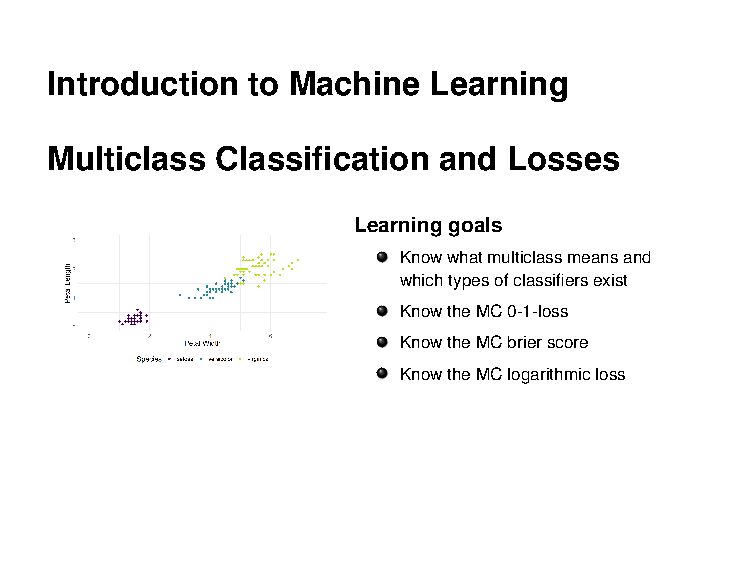
\includepdf[pages=-]{../slides-pdf/slides-mc-losses.pdf}

\subsection{Softmax Regression}
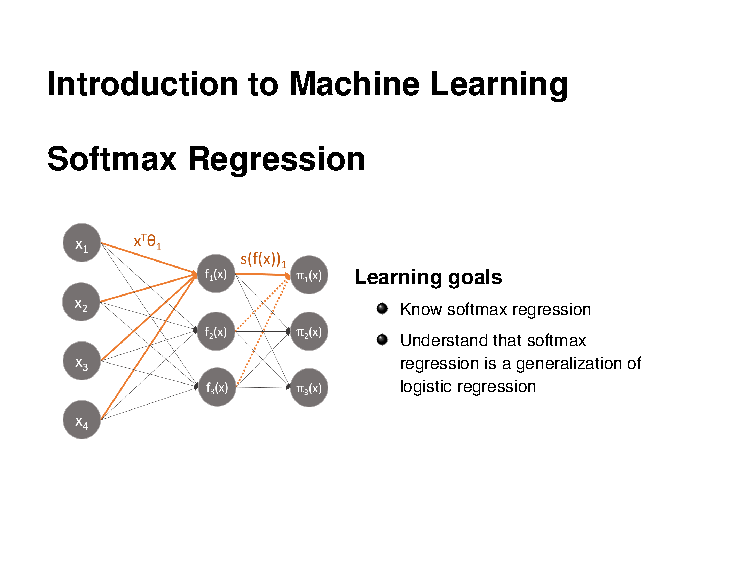
\includepdf[pages=-]{../slides-pdf/slides-mc-softmax-regression.pdf}

\subsection{One-vs-Rest and One-vs-One}
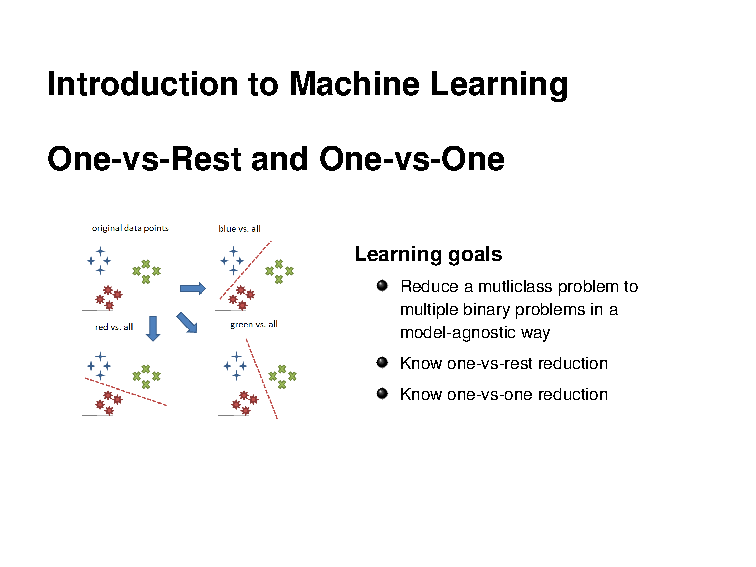
\includepdf[pages=-]{../slides-pdf/slides-mc-binary-reduction.pdf}

\subsection{Designing Codebooks and ECOC}
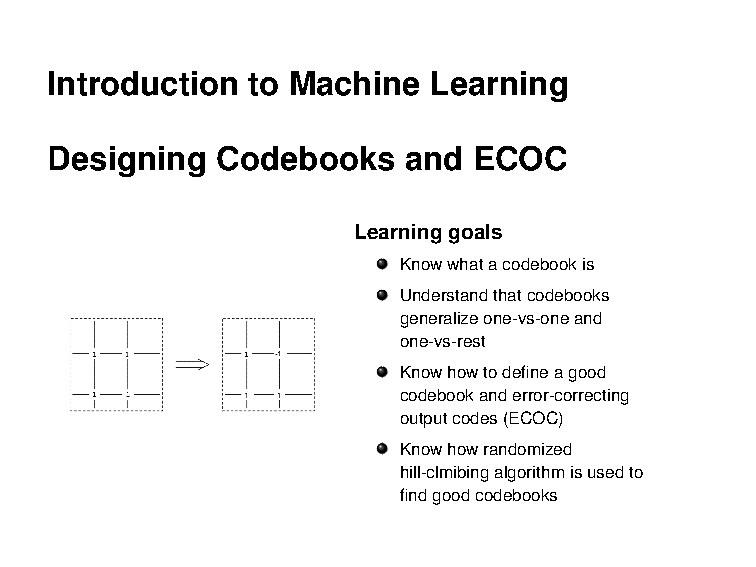
\includepdf[pages=-]{../slides-pdf/slides-mc-codebooks.pdf}




\section{Information Theory}
%Suggested order of slides
% slides-info-entropy
% slides-info-diffent
% slides-info-sourcecoding
% slides-info-kl
% slides-info-cross-entropy-kld
% slides-info-ml
% slides-info-mutual-info

\subsection{Entropy}
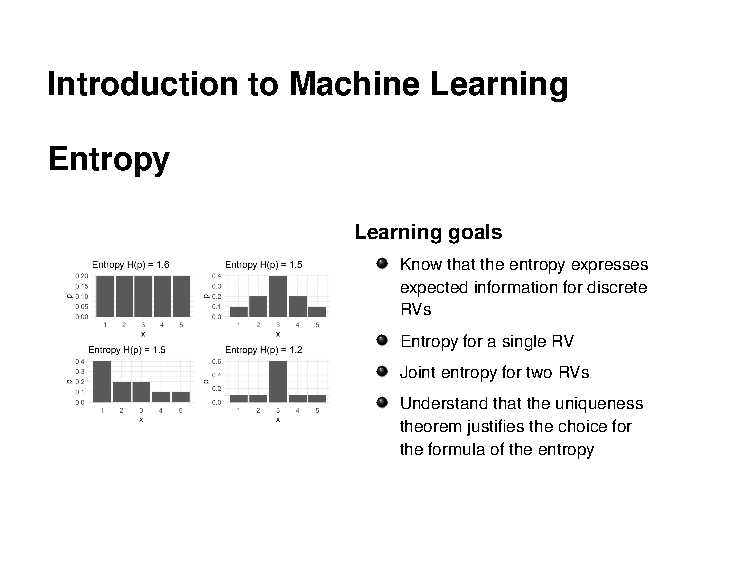
\includepdf[pages=-]{../slides-pdf/slides-info-entropy.pdf}

\subsection{Differential Entropy}
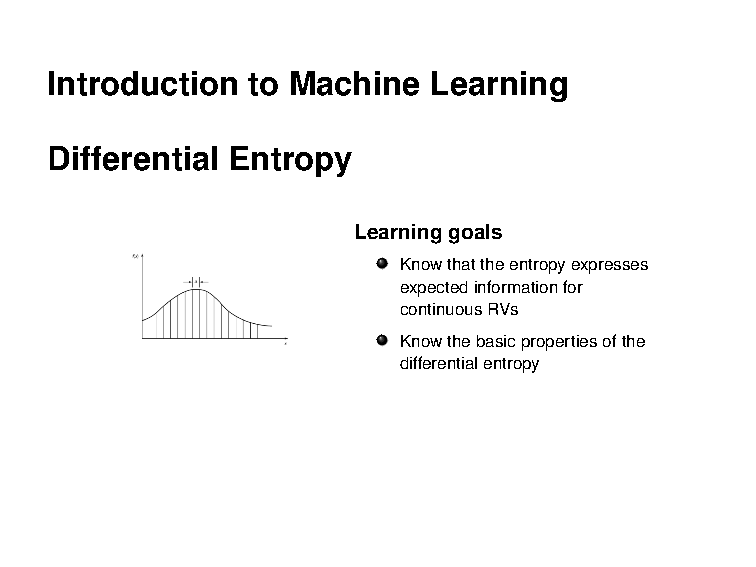
\includepdf[pages=-]{../slides-pdf/slides-info-diffent.pdf}

\subsection{Entropy and Optimal Code Length}
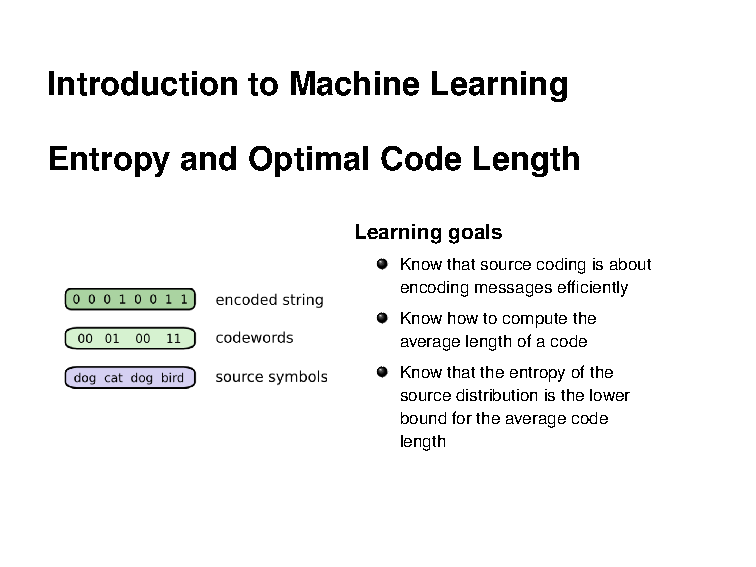
\includepdf[pages=-]{../slides-pdf/slides-info-sourcecoding.pdf}

\subsection{Kullback-Leibler Divergence}
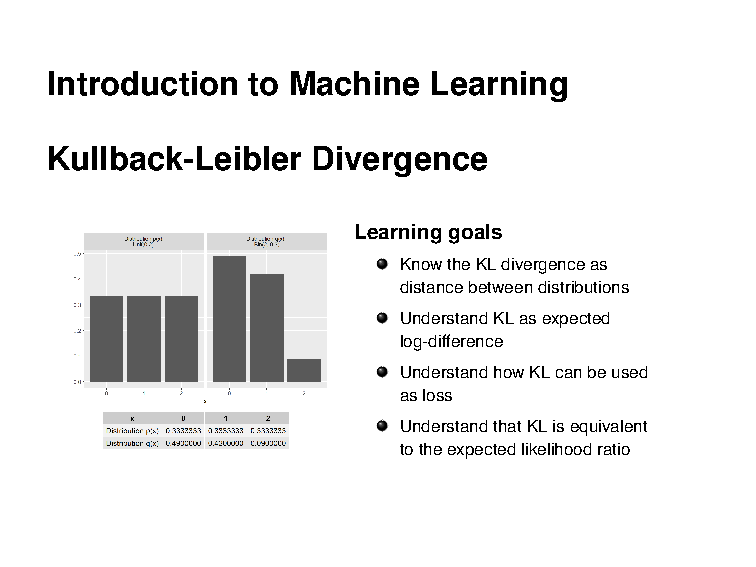
\includepdf[pages=-]{../slides-pdf/slides-info-kl.pdf}

\subsection{Cross-Entropy, KL and Source Coding}
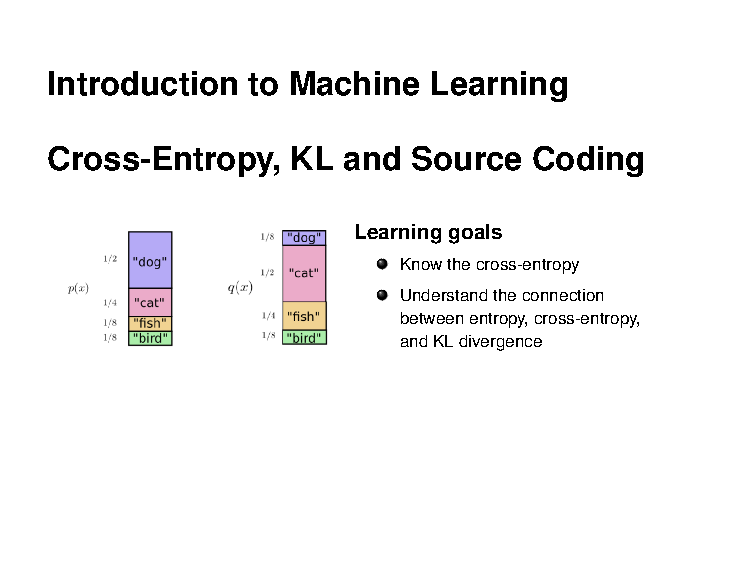
\includepdf[pages=-]{../slides-pdf/slides-info-cross-entropy-kld.pdf}

\subsection{Information Theory for Machine Learning}
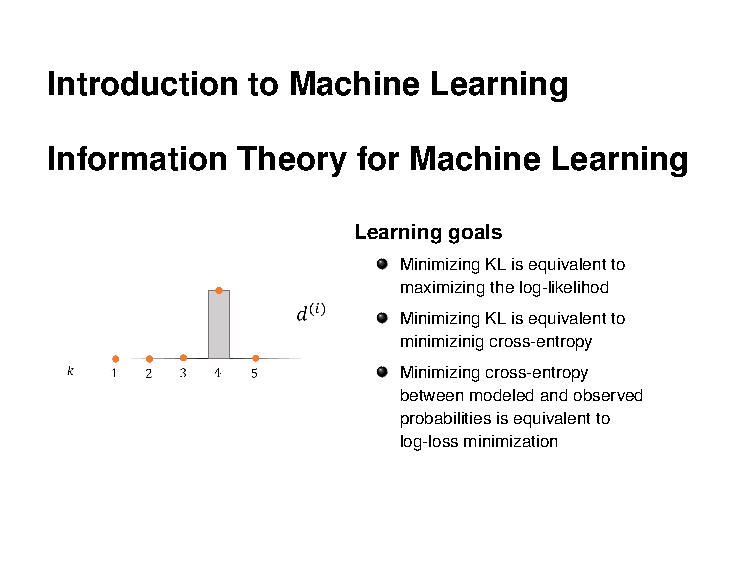
\includepdf[pages=-]{../slides-pdf/slides-info-ml.pdf}

\subsection{Joint Entropy and Mutual Information}
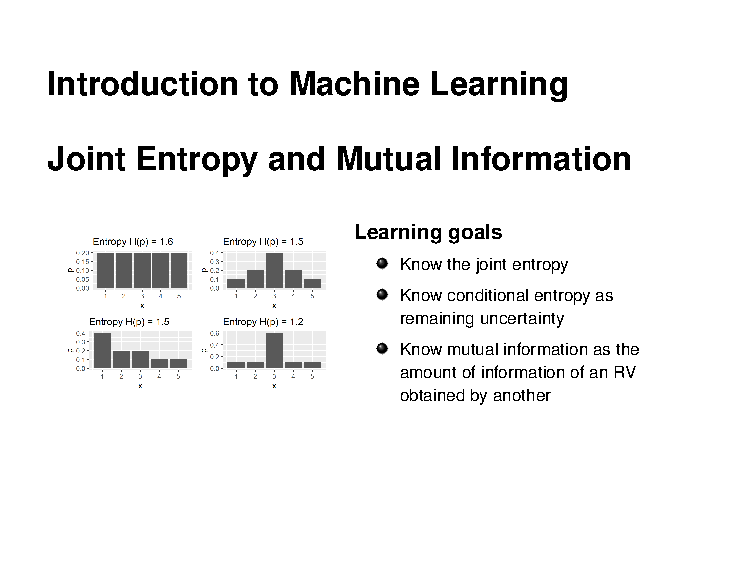
\includepdf[pages=-]{../slides-pdf/slides-info-mutual-info.pdf}




\section{Curse of Dimensionality}
%Suggested order of slides
% slides-cod.tex
% slides-cod-examples.tex


\subsection{Curse of Dimensionality}
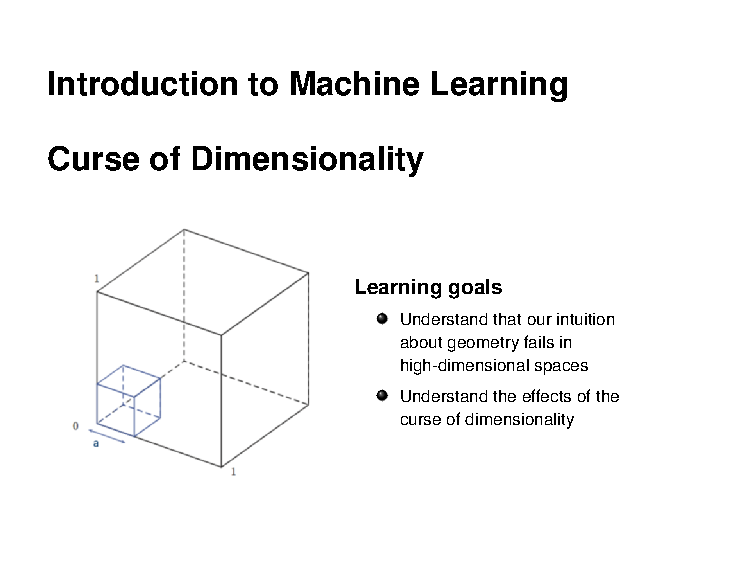
\includepdf[pages=-]{../slides-pdf/slides-cod.pdf}

\subsection{Curse of Dimensionality - Examples}
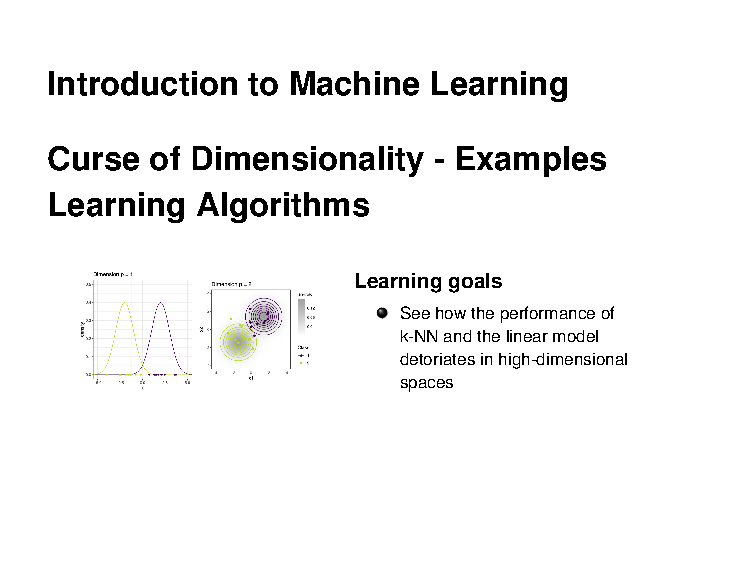
\includepdf[pages=-]{../slides-pdf/slides-cod-examples.pdf}



\section{Hypothesis Space}
%Suggested order of slides
% slides-info-entropy
% slides-info-diffent
% slides-info-sourcecoding
% slides-info-kl
% slides-info-cross-entropy-kld
% slides-info-ml
% slides-info-mutual-info


\subsection{Entropy}
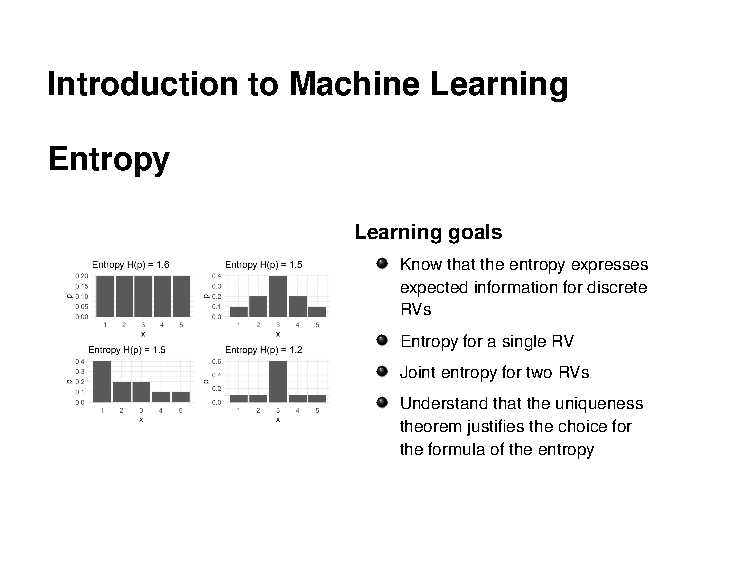
\includepdf[pages=-]{../slides-pdf/slides-info-entropy.pdf}

\subsection{Differential Entropy}
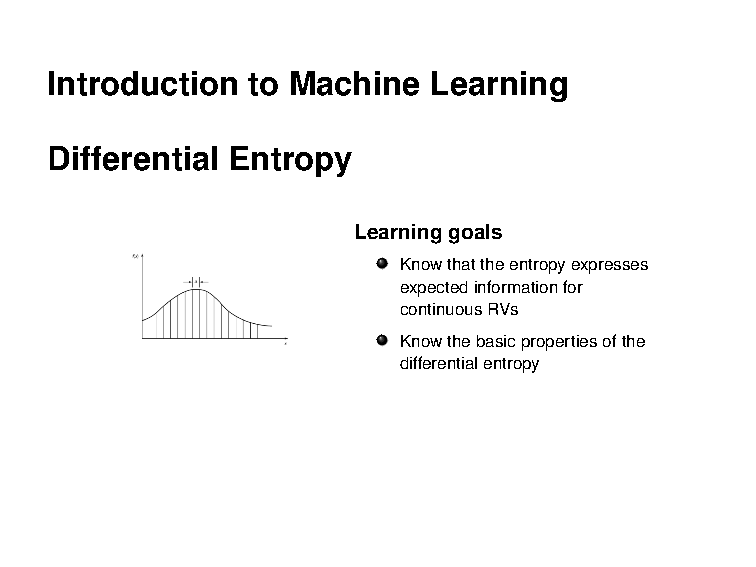
\includepdf[pages=-]{../slides-pdf/slides-info-diffent.pdf}

\subsection{Entropy and Optimal Code Length}
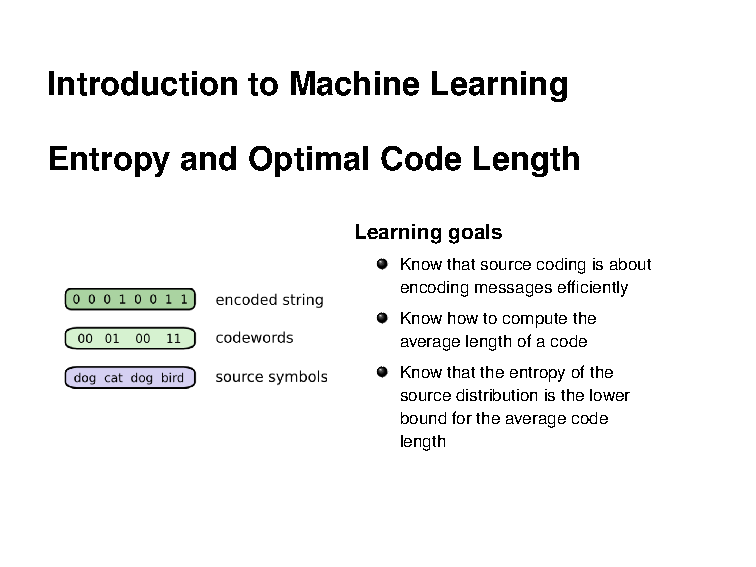
\includepdf[pages=-]{../slides-pdf/slides-info-sourcecoding.pdf}

\subsection{Kullback-Leibler Divergence}
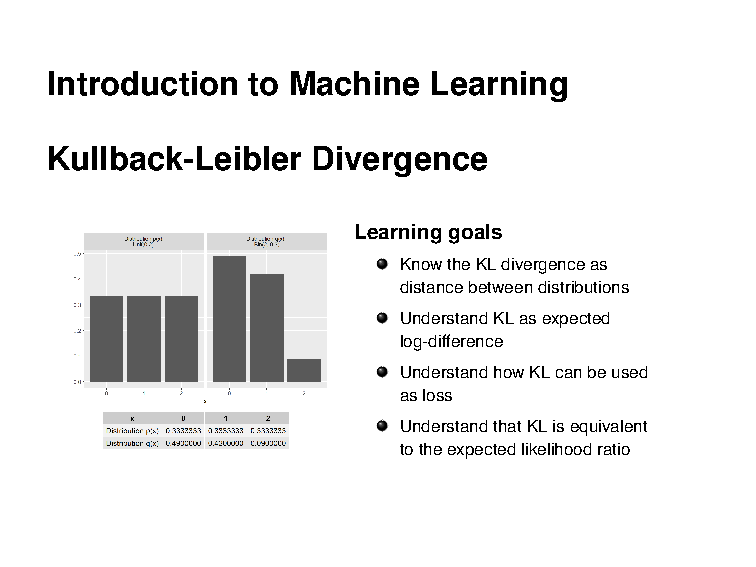
\includepdf[pages=-]{../slides-pdf/slides-info-kl.pdf}

\subsection{Cross-Entropy, KL and Source Coding}
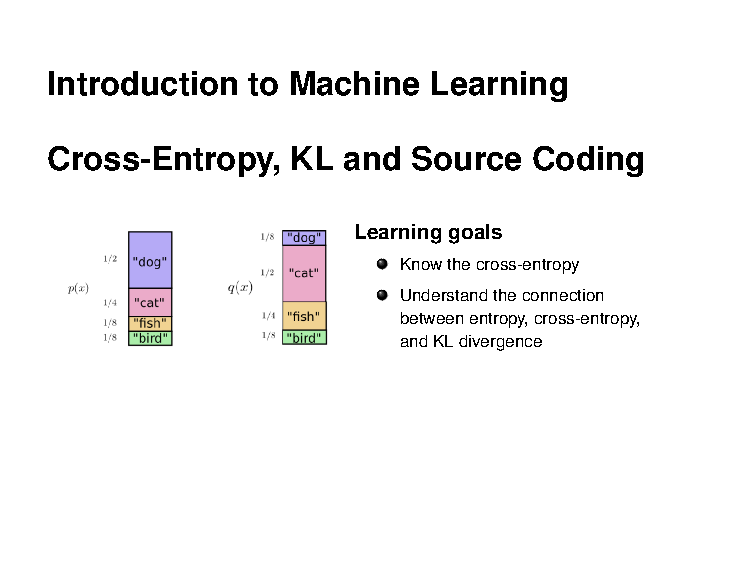
\includepdf[pages=-]{../slides-pdf/slides-info-cross-entropy-kld.pdf}

\subsection{Information Theory for Machine Learning}
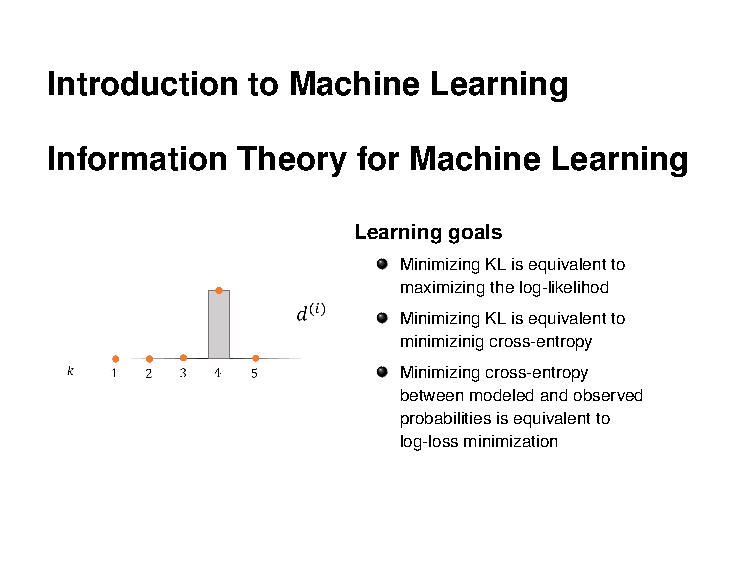
\includepdf[pages=-]{../slides-pdf/slides-info-ml.pdf}

\subsection{Joint Entropy and Mutual Information}
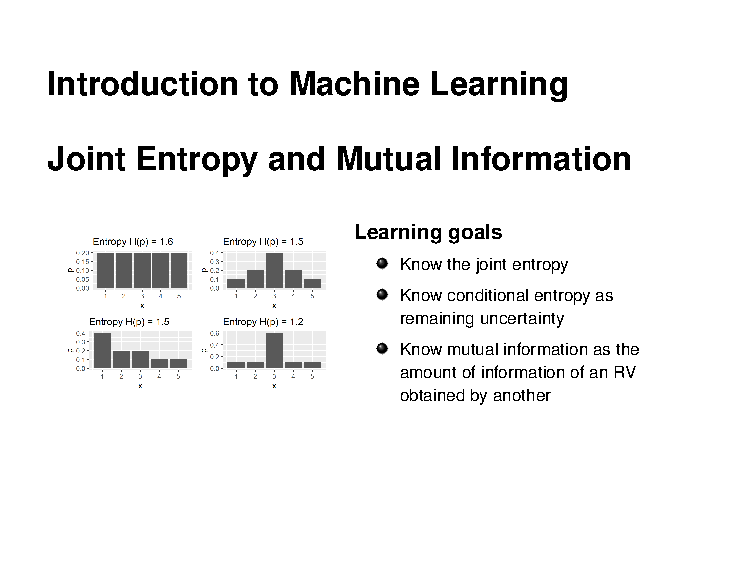
\includepdf[pages=-]{../slides-pdf/slides-info-mutual-info.pdf}




\section{Regularization}
%Suggested order of slides
% slides-regu-intro
% slides-regu-l1l2
% slides-regu-l1vsl2
% slides-regu-enetlogreg
% slides-regu-underdetermined
% slides-regu-l0
% slides-regu-nonlin-bayes
% slides-regu-geom-l2-wdecay
% slides-regu-geom-l1
% slides-regu-early-stopping


\subsection{Introduction to Regularization}
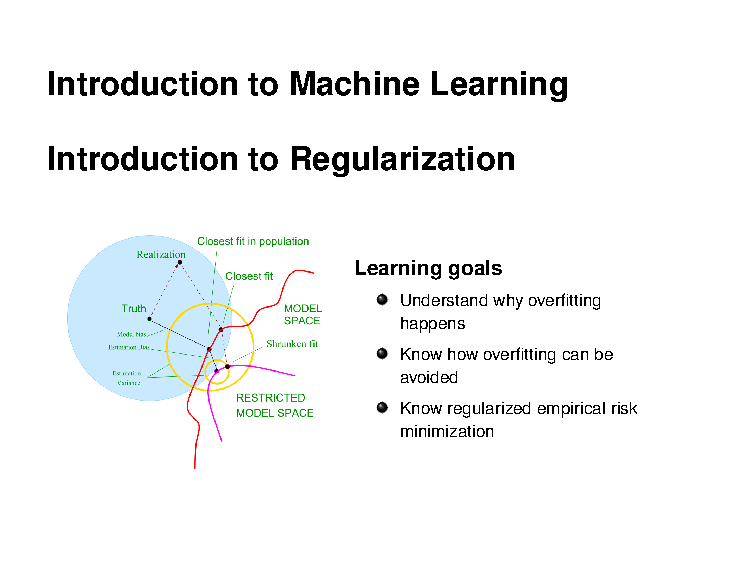
\includepdf[pages=-]{../slides-pdf/slides-regu-intro.pdf}

\subsection{Lasso and Ridge Regression}
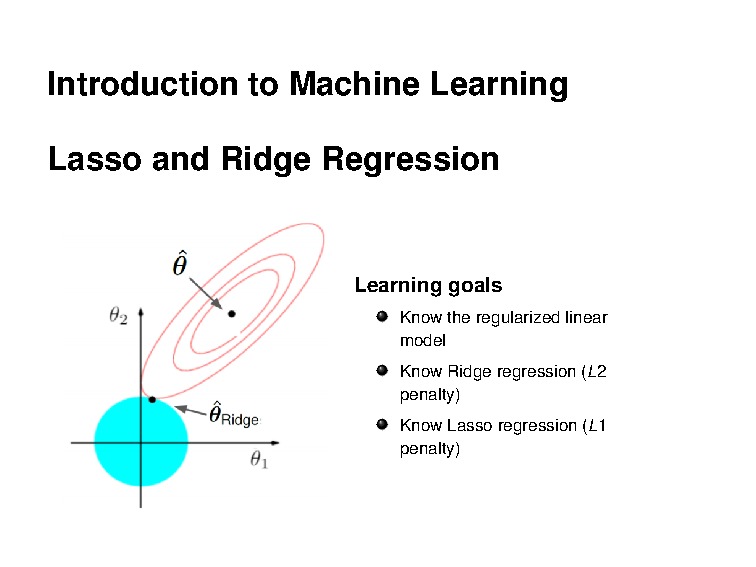
\includepdf[pages=-]{../slides-pdf/slides-regu-l1l2.pdf}

\subsection{Lasso vs. Ridge Regression}
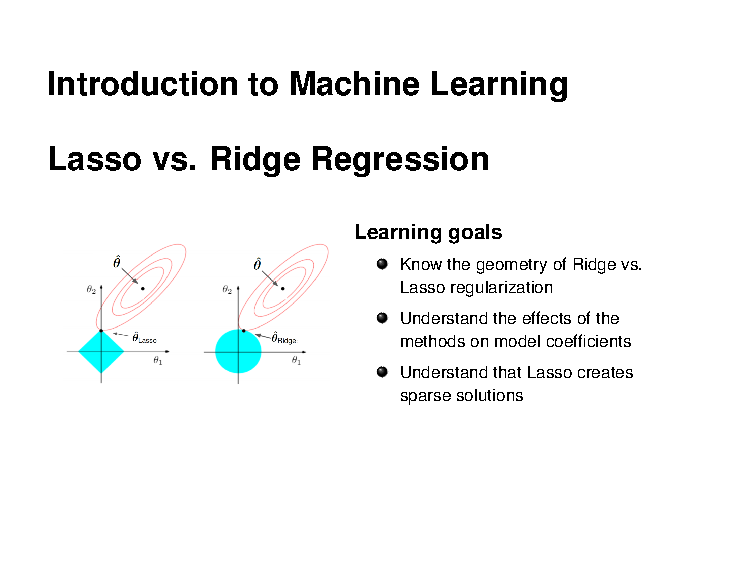
\includepdf[pages=-]{../slides-pdf/slides-regu-l1vsl2.pdf}

\subsection{Elastic Net and Regularization for GLMs}
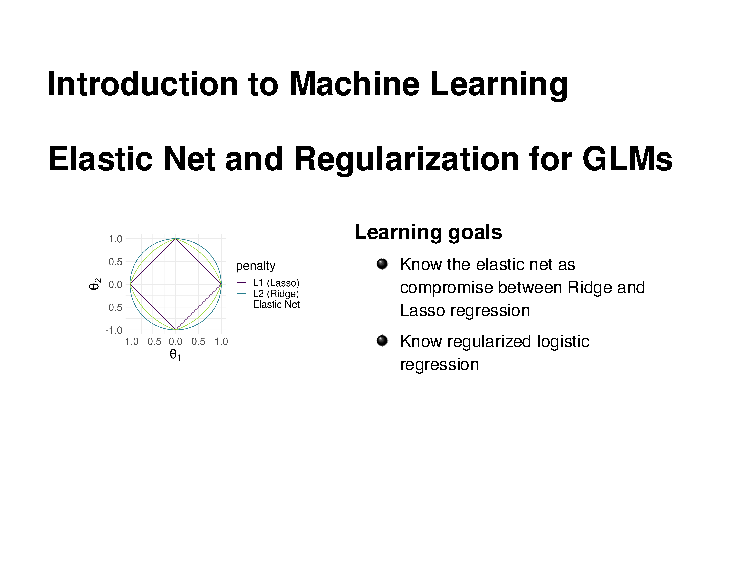
\includepdf[pages=-]{../slides-pdf/slides-regu-enetlogreg.pdf}

\subsection{Regularization for Underdetermined Problem}
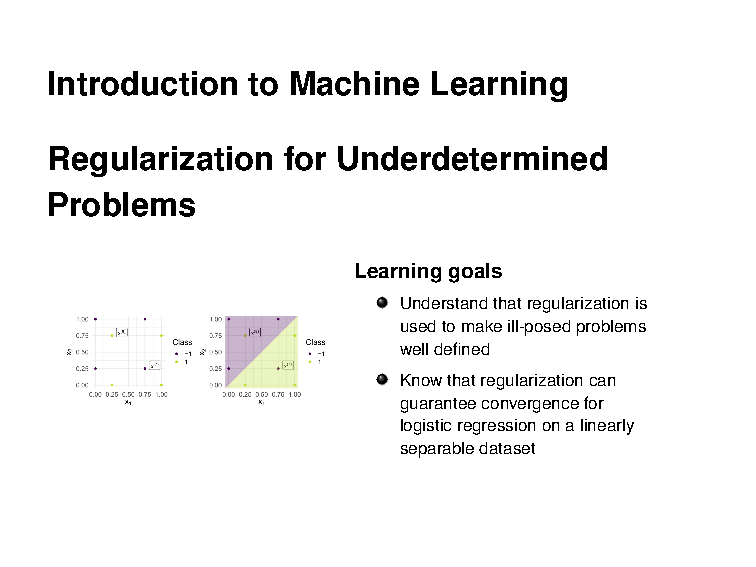
\includepdf[pages=-]{../slides-pdf/slides-regu-underdetermined.pdf}

\subsection{L0 Regularization}
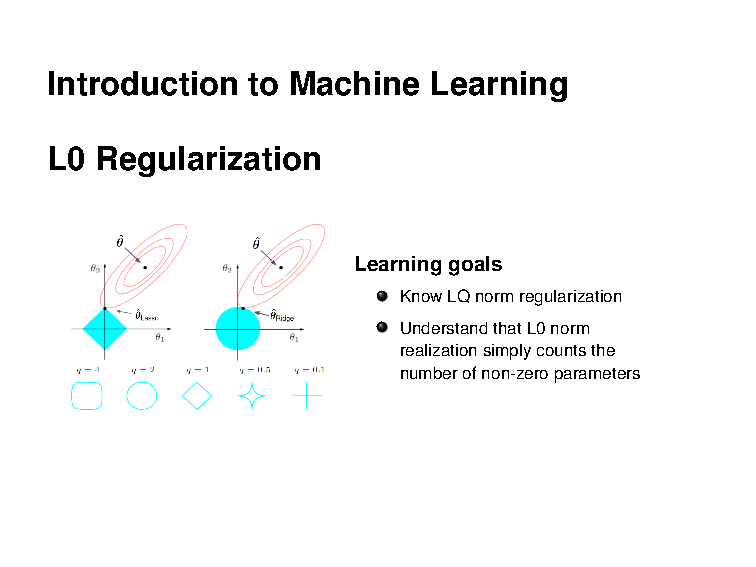
\includepdf[pages=-]{../slides-pdf/slides-regu-l0.pdf}

\subsection{Nonlinear and Bayes}
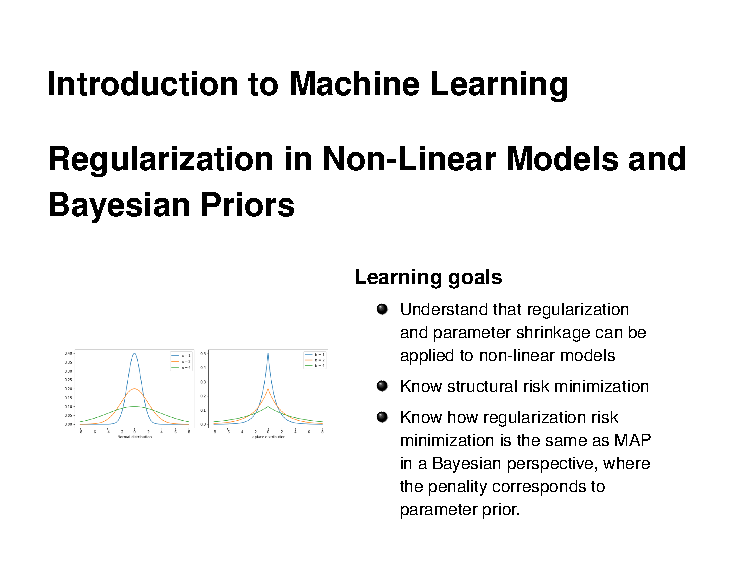
\includepdf[pages=-]{../slides-pdf/slides-regu-nonlin-bayes.pdf}

\subsection{Geometric Analysis of L2-Regularization and Weight Decay}
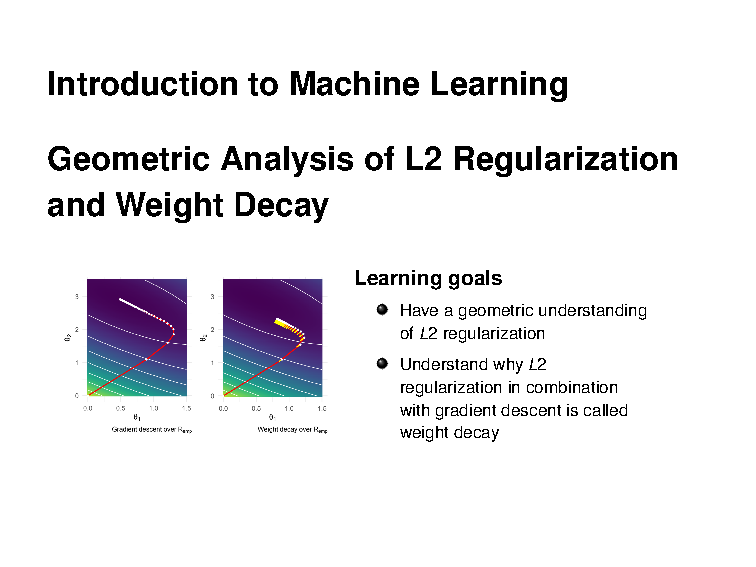
\includepdf[pages=-]{../slides-pdf/slides-regu-geom-l2-wdecay.pdf}

\subsection{Geometric Analysis of L1-regularization}
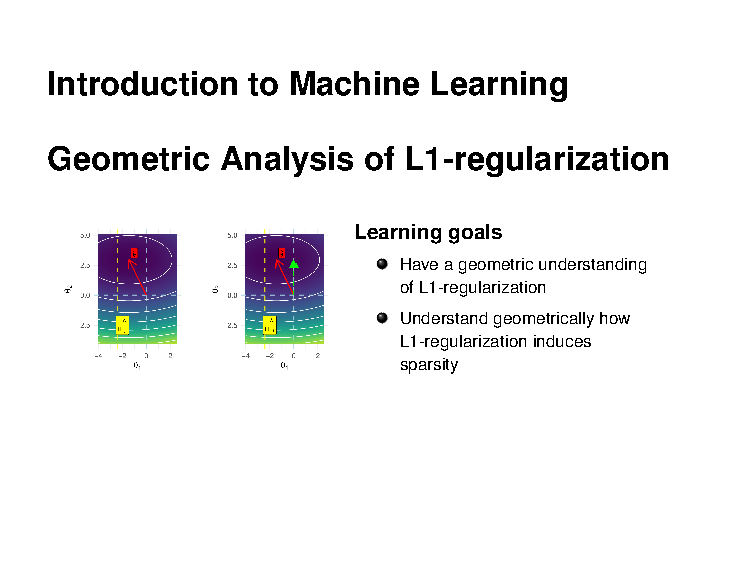
\includepdf[pages=-]{../slides-pdf/slides-regu-geom-l1.pdf}

\subsection{Early Stopping}
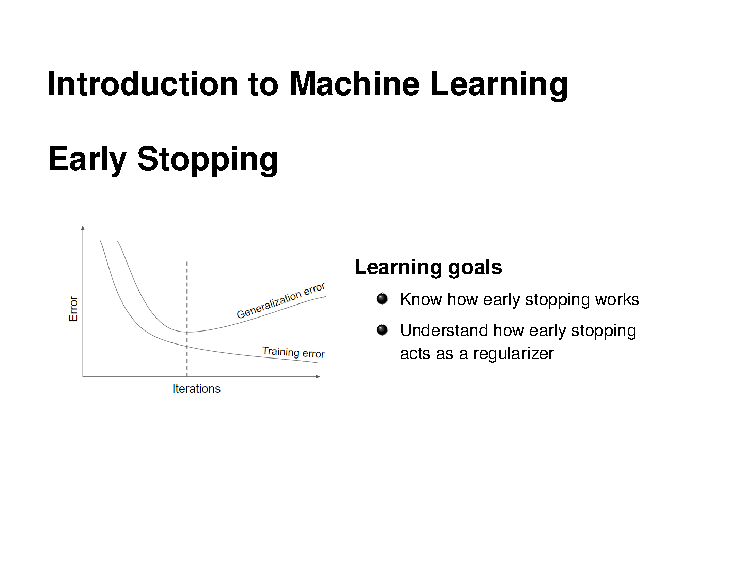
\includepdf[pages=-]{../slides-pdf/slides-regu-early-stopping.pdf}


\section{Linear Support Vector Machine}
%Suggested order of slides
% slides-linsvm-hard-margin
% slides-linsvm-hard-margin-dual
% slides-linsvm-soft-margin
% slides-linsvm-erm
% slides-linsvm-optimization

\subsection{Linear Hard Margin SVM}
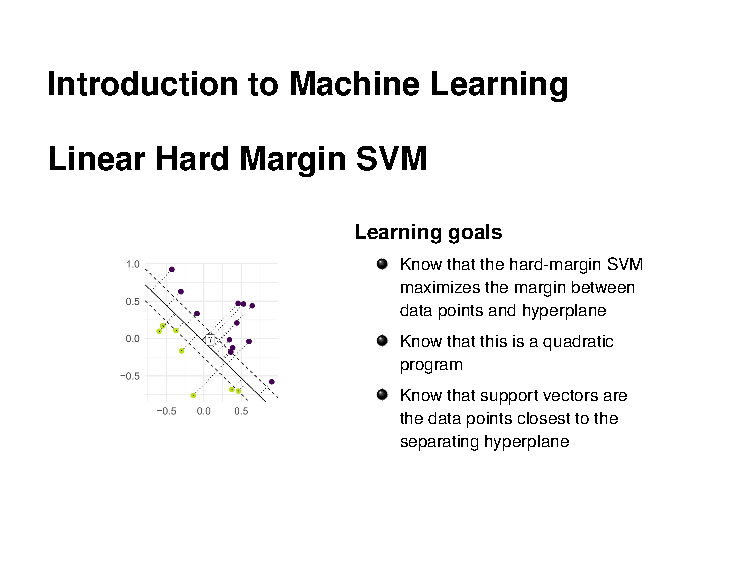
\includepdf[pages=-]{../slides-pdf/slides-linsvm-hard-margin.pdf}

\subsection{Hard-Margin SVM Dual}
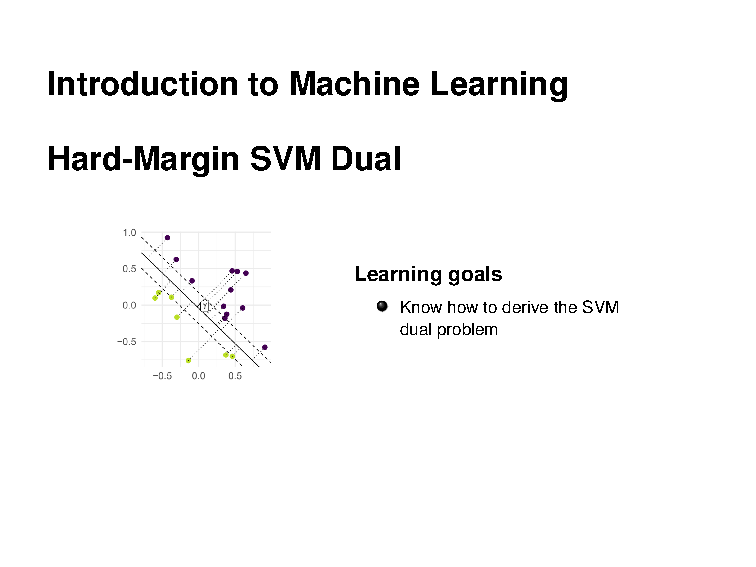
\includepdf[pages=-]{../slides-pdf/slides-linsvm-hard-margin-dual.pdf}

\subsection{Soft-Margin SVM}
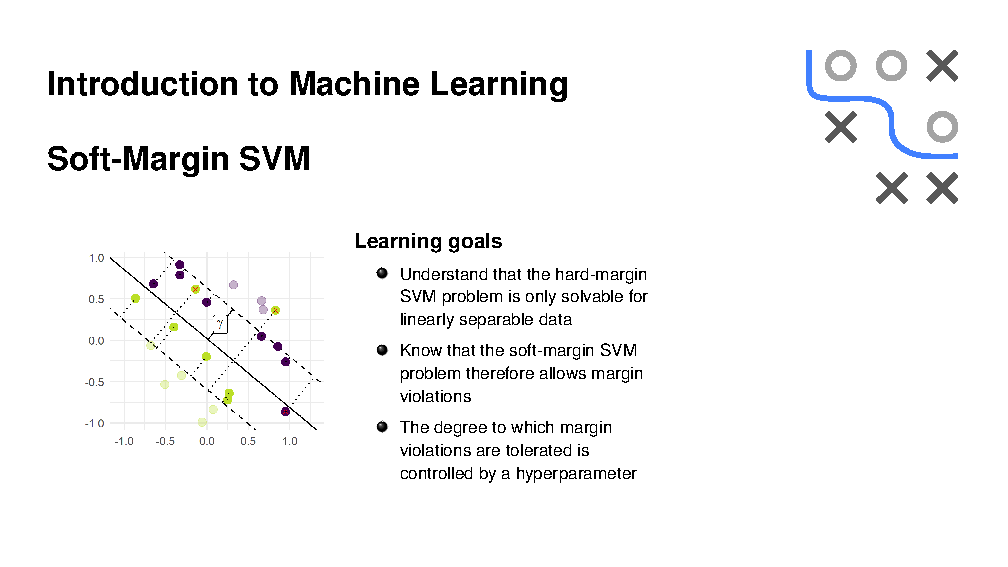
\includepdf[pages=-]{../slides-pdf/slides-linsvm-soft-margin.pdf}

\subsection{SVMs and Empirical Risk Minimization}
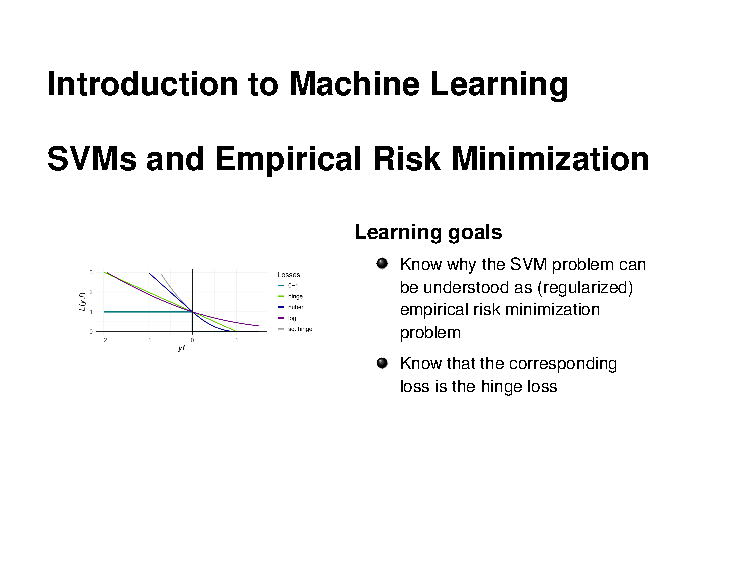
\includepdf[pages=-]{../slides-pdf/slides-linsvm-erm.pdf}

\subsection{Support Vector Machine Training}
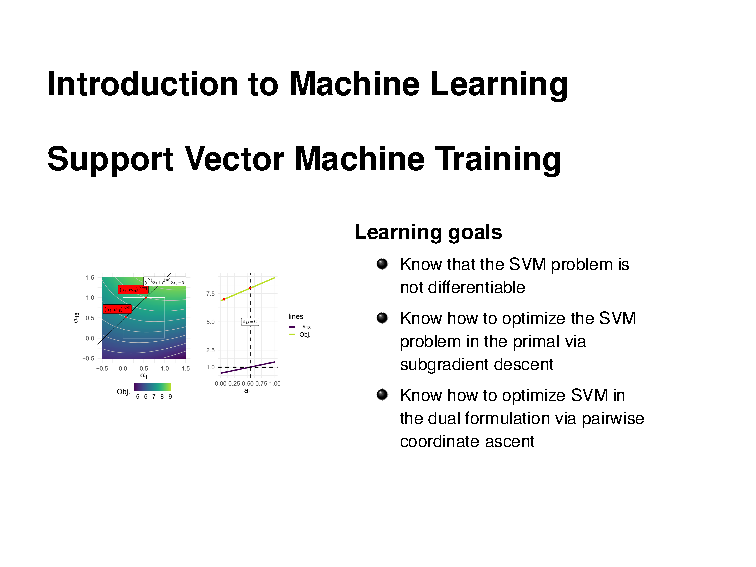
\includepdf[pages=-]{../slides-pdf/slides-linsvm-optimization.pdf}



\section{Nonlinear Support Vector Machine}
%Suggested order of slides
% slides-nonlinsvm-featuregen
% slides-nonlinsvm-kernel-trick
% slides-nonlinsvm-kernel-poly
% slides-nonlinsvm-rkhs-repr
% slides-nonlinsvm-kernel-rbf
% slides-nonlinsvm-modelsel
% slides-nonlinsvm-uniapprox


\subsection{Feature Generation for Nonlinear Separation}
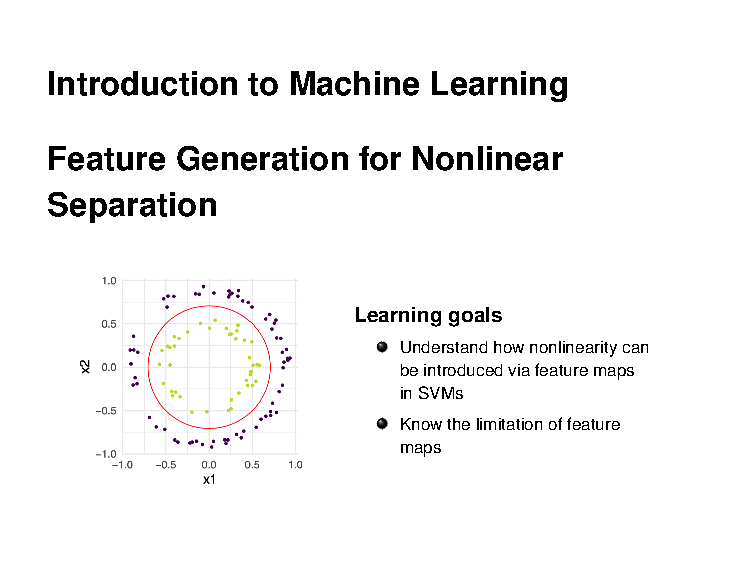
\includepdf[pages=-]{../slides-pdf/slides-nonlinsvm-featuregen.pdf}

\subsection{The Kernel Trick}
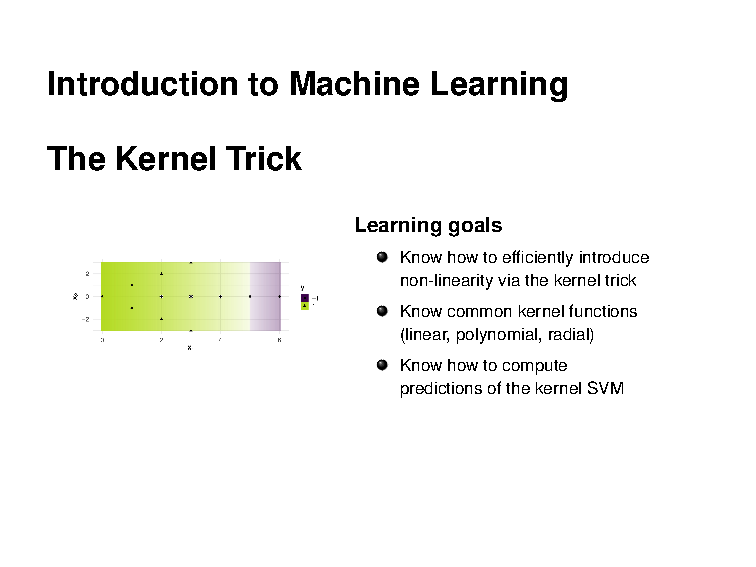
\includepdf[pages=-]{../slides-pdf/slides-nonlinsvm-kernel-trick.pdf}

\subsection{The Polynomial Kernel}
\includepdf[pages=-]{../slides-pdf/slides-nonlinsvm-kernel-poly.pdf}

\subsection{Reproducing Kernel Hilbert Space and Representer Theorem}
\includepdf[pages=-]{../slides-pdf/slides-nonlinsvm-rkhs-repr.pdf}

\subsection{The Gaussian RBF Kernel}
\includepdf[pages=-]{../slides-pdf/slides-nonlinsvm-kernel-rbf.pdf}

\subsection{SVM Model Selection}
\includepdf[pages=-]{../slides-pdf/slides-nonlinsvm-modelsel.pdf}

\subsection{Details on Support Vector Machines}
\includepdf[pages=-]{../slides-pdf/slides-nonlinsvm-uniapprox.pdf}





\section{Gaussian Processes}
%Suggested order of slides
% slides-bayes-lm.tex
% slides-gp-basic.tex
% slides-gp-covariance.tex
% slides-gp-prediction.tex
% slides-gp-training.tex
% slides-gp-mean.tex

% not included: 
% slides-x-covariance-adv.tex
% slides-x-gp-additional.tex
% slides-x-gp-classification.tex

\subsection{Bayes LM}
\includepdf[pages=-]{../slides-pdf/slides-gp-bayes-lm.pdf}
\subsection{Gaussian Processes - Basics}
\includepdf[pages=-]{../slides-pdf/slides-gp-basic.pdf}
\subsection{Gaussian Processes - Covariance}
\includepdf[pages=-]{../slides-pdf/slides-gp-covariance.pdf}
\subsection{Gaussian Processes - Prediction}
\includepdf[pages=-]{../slides-pdf/slides-gp-prediction.pdf}
\subsection{Gaussian Processes - Training}
\includepdf[pages=-]{../slides-pdf/slides-gp-training.pdf}
\subsection{Gaussian Processes - Mean}
\includepdf[pages=-]{../slides-pdf/slides-gp-mean.pdf}


\section{Boosting}
%Suggested order of slides
% slides-boosting-intro-adaboost
% slides-boosting-gradient-boosting-concept
% slides-boosting-regression-illustrations
% slides-boosting-gbm-regularization
% slides-boosting-gbm-classification
% slides-boosting-gbm-with-trees
% slides-boosting-xgboost
% slides-boosting-comp-boost





\subsection{Introduction to Boosting / AdaBoost}
\includepdf[pages=-]{../slides-pdf/slides-boosting-intro-adaboost.pdf}

\subsection{Gradient Boosting Concept}
\includepdf[pages=-]{../slides-pdf/slides-boosting-gradient-boosting-concept.pdf}

\subsection{Gradient Boosting - Illustration}
\includepdf[pages=-]{../slides-pdf/slides-boosting-regression-illustrations.pdf}

\subsection{Gradient Boosting: Regularization}
\includepdf[pages=-]{../slides-pdf/slides-boosting-gbm-regularization.pdf}

\subsection{Gradient Boosting for Classification}
\includepdf[pages=-]{../slides-pdf/slides-boosting-gbm-classification.pdf}

\subsection{Gradient Boosting with Trees}
\includepdf[pages=-]{../slides-pdf/slides-boosting-gbm-with-trees.pdf}

\subsection{XGBoost}
\includepdf[pages=-]{../slides-pdf/slides-boosting-xgboost.pdf}

\subsection{Componentwise gradient boostin}
\includepdf[pages=-]{../slides-pdf/slides-boosting-comp-boost.pdf}










\end{document}
